\documentclass[ngerman,compress]{beamer}

\mode<presentation>
{
  \useoutertheme[footline=titleinstituteauthor]{c4}
  \useinnertheme{circles}
  \usecolortheme{c4}
  %\setbeamercovered{transparent}
  \setbeamercovered{highly dynamic}
}

\usepackage{babel}
\usepackage[utf8]{luainputenc}
\usepackage{fontspec}
\usepackage{listings}
\usepackage{color}
\usepackage{mathtools}

% Multimedia
%\usepackage{multimedia}

% sets the listings style
\definecolor{sh_comment}{rgb}{0.12, 0.38, 0.18 } %adjusted, in Eclipse: {0.25, 0.42, 0.30 } = #3F6A4D
\definecolor{sh_keyword}{rgb}{0.3, 0.3, 0.875}  % #5F1441
\definecolor{sh_string}{rgb}{0.875, 0.85, 0.11} % #101AF9

\lstset{basicstyle=\tiny\ttfamily,
	showspaces=false,
	showtabs=false,
	showstringspaces=false,
	columns=fullflexible,
	stringstyle=\color{sh_string},
	keywordstyle=\color{sh_keyword}\bfseries,
	commentstyle=\color{sh_comment}\itshape
	}

\title[STM32 - I2C - u23 2013]
{\textbf{STM32 - I2C}\\u23 2013}

\author[andy <andy@koeln.ccc.de>]
{andy, florob, gordin, ike, meise, tobix, zakx}

\institute[Chaos Computer Club Cologne]
{
Chaos Computer Club Cologne e.V.\\
http://koeln.ccc.de \\
}

\date{Cologne\\2013-11-11}

\pgfdeclareimage[height=1cm]{barcode}{./c4-logo_narr}
\logo{\pgfuseimage{barcode}}


% Folgendes sollte gelC6scht werden, wenn man nicht am Anfang jedes
% Unterabschnitts die Gliederung nochmal sehen möchte.
%\AtBeginSection[]
%{
%  \begin{frame}<beamer>
%    \frametitle{Gliederung}
%    \tableofcontents[currentsection,currentsubsection]
%  \end{frame}
%}

% Falls Aufzählungen immer schrittweise gezeigt werden sollen, kann
% folgendes Kommando benutzt werden:
%\beamerdefaultoverlayspecification{<+->}


\begin{document}

\begin{frame}
  \titlepage
\end{frame}

\AtBeginSubsection

\begin{frame}
  \tableofcontents
  % Die Option [pausesections] könnte nützlich sein.
\end{frame}

\section {Allgemeines}

\begin{frame}
	\frametitle{Teile!}
	\begin{center}
	\huge{Ey! Psst! Brauchste Teile?} \\
	\large{Liegen hier vorne auf dem Tisch}
	\end{center}
\end{frame}

\section{Hardware}

\subsection{I2C Hardware und Busprotokoll}

\begin{frame}
	\frametitle{I2C}
	\begin{itemize}
		\item I2C = Inter-integrated Circuit (I-Quadrat-C oder I-squared-C gesprochen)
		\item Markenname von Philips, sonst TWI = Two Wire Interface
		\item 2-Draht Bussystem für Bausteine die in einem geschlossenen System zusammen arbeiten (selbe Platine, selbes Gehäuse, ...)
		\item Alle Kommunikation geht von einem oder mehreren Mastern aus, Slavebausteine machen nie etwas von sich aus
		\item Verschiedene Geschwindigkeiten: 100kHz, 400kHz (fast mode), 1MHz (fast mode plus) und 3,4MHz (high speed mode)
		\item 7- oder 10-Bit lange Adressen für Slavebausteine
	\end{itemize}
\end{frame}

\begin{frame}
	\frametitle{I2C}
	\begin{itemize}
		\item Zwei Leitungen:
		\begin{enumerate}
			\item SCL = Clock
			\item SDA = Data
		\end{enumerate}
		\item Beides Open-Drain-Leitungen (wir erinnern uns an die GPIOs)
		\item Pull-Ups müssen eigentlich auf Leitungslänge, Anzahl Teilnehmer, Geschwindigkeit etc. abgestimmt werden
		\item In der Praxis: Nehmt was zwischen 4,7K und 10K
		\item Standard scheint so 4,7K zu sein
		\item Mein großer Quadrocopter hat 2,2K, tut auch...
		\item Die HMC5883L-Kompassboards haben 2,2K
	\end{itemize}
\end{frame}

\begin{frame}
	\frametitle{I2C}
	So sieht son Bus aus:
	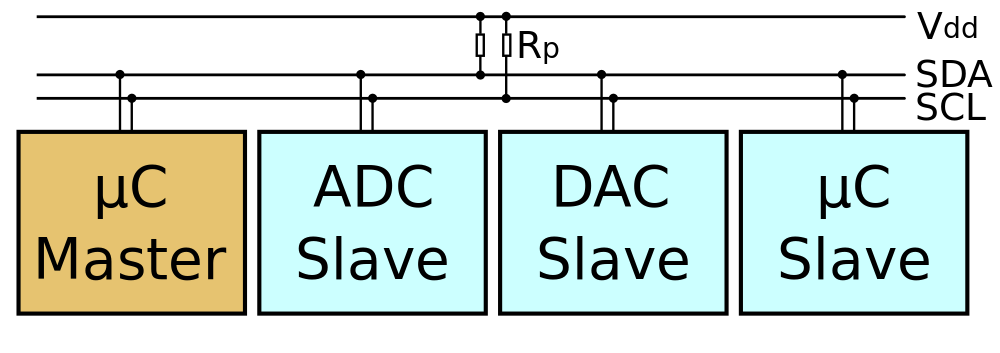
\includegraphics[width=4in]{I2C.png}
\end{frame}

\begin{frame}
	\frametitle{I2C}
	\begin{itemize}
		\item SPI war einfach gestrickt: Daten rein und raus bei Clockgewackel, nur eine Richtung pro Datenleitung
		\item I2C ist etwas komplizierter, da hier ein Protokoll gesprochen werden muss
		\item Nur eine Datenleitung zum lesen und schreiben und Adressen für Slaves
	\end{itemize}
\end{frame}

\begin{frame}
	\frametitle{I2C Protokoll}
	\begin{itemize}
		\item 4 spezielle Bus-Conditions:
		\begin{enumerate}
			\item START
			\item STOP
			\item ACK
			\item NACK
		\end{enumerate}
	\end{itemize}
\end{frame}

\begin{frame}
	\frametitle{START- und STOP-Condition}
	\begin{itemize}
		\item START wird genutzt um den Bus zu aktivieren und eine Transaktion zu starten
		\item STOP beendet eine Transaktion egal in welchem Zustand und gibt den Bus wieder frei
		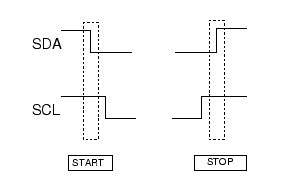
\includegraphics[width=3in]{i2c-tutorial-star-stop}
	\end{itemize}
\end{frame}

\begin{frame}
	\frametitle{ACK und NACK}
	\begin{itemize}
		\item ACK und NACK sind Bits die zu bestimmten Zeitpunkten im Komunikationsablauf gesendet werden
		\item ACK bestätigt empfang eines Bytes
		\item NACK bestätigt zwar den Empfang, signalisiert aber gleichzeitig einen Fehler oder ähnliches
		\item Nack einem NACK vom Slave kann der Master nur ein STOP oder Repeated START senden
	\end{itemize}
\end{frame}

\begin{frame}
	\frametitle{Transfer Master -> Slave}
	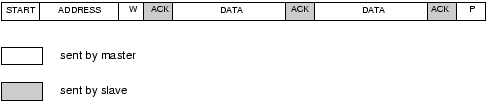
\includegraphics[width=4in]{i2c-tutorial-master-slave}
	\begin{enumerate}
		\item START senden
		\item 7-Bit Adresse senden
		\item Read/Write-Bit senden (1=Read, 0=Write)
		\item Auf ein ACK vom Slave warten
		\item 8 Bit senden
		\item Auf ACK-Bit warten
		\item ...
		\item 8 Bit senden
		\item Auf ACK-Bit warten
		\item STOP senden
	\end{enumerate}
\end{frame}

\begin{frame}
	\frametitle{Transfer Slave -> Master}
	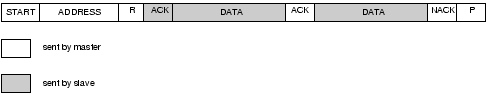
\includegraphics[width=4in]{i2c-tutorial-slave-master}
	\begin{enumerate}
		\item START senden
		\item 7-Bit Adresse senden
		\item Read/Write-Bit senden (1=Read, 0=Write)
		\item Auf ein ACK vom Slave warten
		\item 8 Bit empfangen
		\item ACK-Bit Senden
		\item ...
		\item 8 Bit empfangen
		\item NACK-Bit senden
		\item STOP senden
	\end{enumerate}
\end{frame}

\begin{frame}
	\frametitle{Repeated Start}
	\begin{itemize}
		\item Wir können also jetzt lesen und schreiben
		\item Aber was ist, wenn wir erst schreiben wollen und dann lesen?
	\end{itemize}
	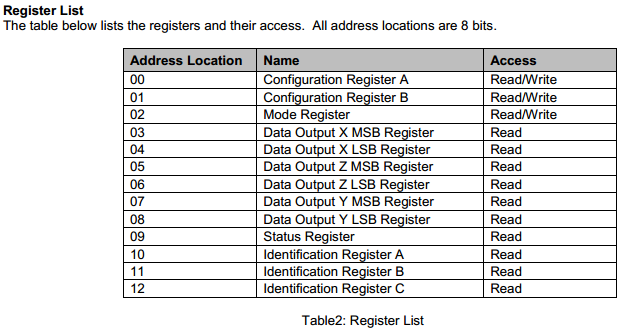
\includegraphics[width=4in]{hmc_regs}
\end{frame}

\begin{frame}
	\frametitle{Repeated Start}
	\begin{itemize}
		\item Man schreibt die Registeradresse in einer ersten Transaktion
		\item Und liest dann den 8-Bit Wert
		\item Der Slave sollte dann den Registerinhalt zurückliefern
		\item VORSICHT! Das muss nicht so sein, in der Regel liest und schreibt man aber so Register
	\end{itemize}
\end{frame}

\begin{frame}
	\frametitle{Repeated Start}
	\begin{itemize}
		\item Dumm nur: Bus wird zwischen dem Write der Registeradresse wieder freigegeben
		\item In der Zwischenzeit kann such ein anderer Master den Bus unter den Nagel reißen
		\item Der schreibt dann eine Registeradresse auf dem selben Slave -> Wir lesen dann einen falschen Wert
	\end{itemize}
\end{frame}

\begin{frame}
	\frametitle{Repeated Start}
	\begin{itemize}
		\item Die Lösung ist Repeated Start
		\item Statt einem STOP sendet man einfach nochmal START
		\item Dann wieder die Slaveadresse und ein R/W-Bit logischerweise jetzt invertiert, da man ja den Modus ändern will
	\end{itemize}
\end{frame}

\begin{frame}
	\frametitle{Write}
	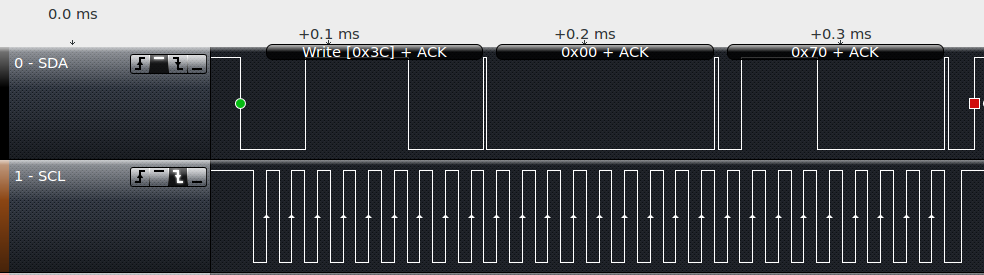
\includegraphics[width=4.5in]{reg_write}
\end{frame}

\begin{frame}
	\frametitle{Write, Repeated Start, Read}
	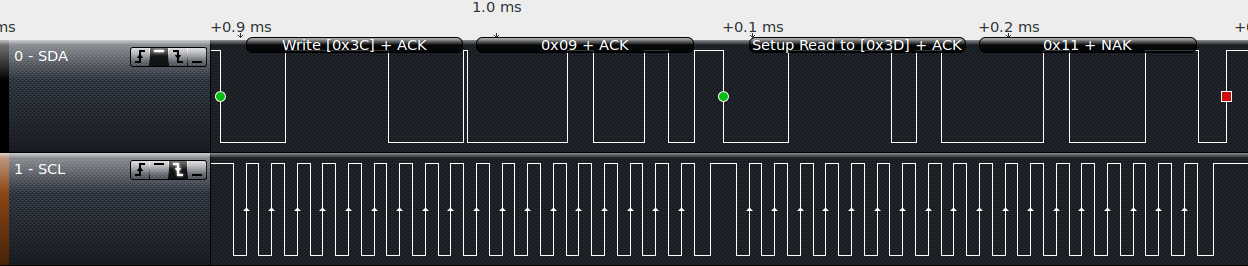
\includegraphics[width=4.5in]{repeated_start}
\end{frame}

\begin{frame}
	\frametitle{Read mehrerer Werte}
	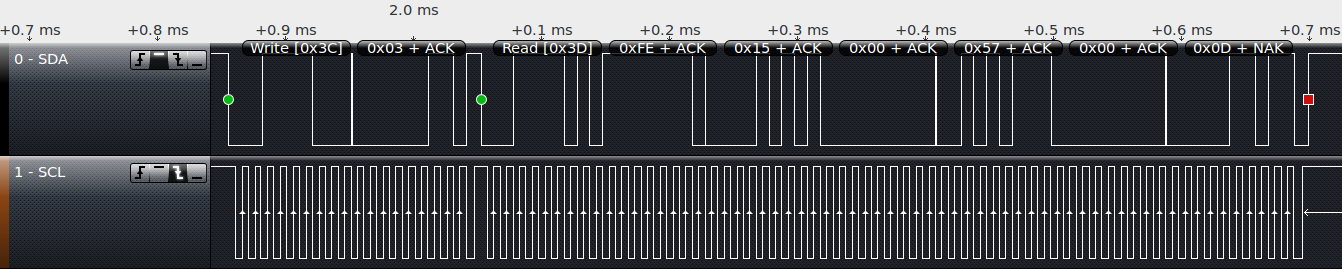
\includegraphics[width=4.5in]{multiread}
\end{frame}

\section{Software}

\subsection{I2C Reden}

\begin{frame} [fragile]
	\frametitle{Konfiguration}
	\begin{lstlisting} [language=C]
// Enable clock for GPIOA and GPIOC peripheral
RCC_AHB1PeriphClockCmd(RCC_AHB1Periph_GPIOA, ENABLE);
RCC_AHB1PeriphClockCmd(RCC_AHB1Periph_GPIOC, ENABLE);

// Set Pin modes for PA8 (SCL)
GPIO_Init(GPIOA, &(GPIO_InitTypeDef){
    .GPIO_Speed = GPIO_Speed_2MHz,
    .GPIO_Mode = GPIO_Mode_AF,		//Not OUT, but AF = Alternate Function
    .GPIO_OType = GPIO_OType_OD,
    .GPIO_PuPd = GPIO_PuPd_NOPULL,	//External pullups, so none here
    .GPIO_Pin = GPIO_Pin_8
});

// Set Pin modes for PC9 (SDA)
GPIO_Init(GPIOC, &(GPIO_InitTypeDef){
    .GPIO_Speed = GPIO_Speed_2MHz,
    .GPIO_Mode = GPIO_Mode_AF,		//Not OUT, but AF = Alternate Function
    .GPIO_OType = GPIO_OType_OD,
    .GPIO_PuPd = GPIO_PuPd_NOPULL,	//External pullups, so none here
    .GPIO_Pin = GPIO_Pin_9
});

//Attach alternate pin functions
GPIO_PinAFConfig(GPIOA, GPIO_PinSource8, GPIO_AF_I2C3);	//SCL
GPIO_PinAFConfig(GPIOC, GPIO_PinSource9, GPIO_AF_I2C3);	//SDA
	\end{lstlisting}
\end{frame}

\begin{frame} [fragile]
	\frametitle{Konfiguration}
	\begin{lstlisting} [language=C, basicstyle=\small]
I2C_Init(I2C3, &(I2C_InitTypeDef){
    .I2C_ClockSpeed = 100000,			//see note above
    .I2C_Mode = I2C_Mode_I2C,			//we want raw I2C, no SMBUS or other stuff
    .I2C_DutyCycle = I2C_DutyCycle_2,	//only relevant for fast mode
    .I2C_OwnAddress1 = 0xEE,			//only relevant for slave mode
    .I2C_AcknowledgedAddress = I2C_AcknowledgedAddress_7bit,	//7-bit addresses, only relevant for slave mode
    .I2C_Ack = I2C_Ack_Disable			//wether or not to acknowledge automatically
});

//Turn that thing on...
I2C_Cmd(I2C3, ENABLE);
	\end{lstlisting}
\end{frame}

\begin{frame} [fragile]
	\frametitle{Register schreiben}
	\begin{lstlisting} [language=C, basicstyle=\small]
I2C_start(I2C3, SLAVE_ADDRESS<<1, I2C_Direction_Transmitter);
I2C_write(I2C3, 0x00); // set pointer to CRA
I2C_write(I2C3, 0x70); // write 0x70 to CRA
I2C_stop(I2C3);
	\end{lstlisting}
\end{frame}

\begin{frame} [fragile]
	\frametitle{Register lesen}
	\begin{lstlisting} [language=C, basicstyle=\small]
//Read Status register, just for the lulz
uint8_t status = 0;
I2C_start(I2C3, SLAVE_ADDRESS<<1, I2C_Direction_Transmitter);
I2C_write(I2C3, 0x09); // set pointer to Status register
I2C_restart(I2C3, SLAVE_ADDRESS<<1, I2C_Direction_Receiver);	//repeated start, now reading
status = I2C_read_nack(I2C3);	//read byte, nack and stop
	\end{lstlisting}
\end{frame}

\begin{frame}
	\frametitle{I2C Beispiel}
	\begin{enumerate}
		\item Eigentlich ist alles was ihr benötigt im \emph{09\_i2c} example
		\item Das Ding redet mit einem HMC5883L I2C-Kompass
		\item Da haben wir leider nur 2 von :(
		\item Ansonsten gibts noch 3 Realtimeclocks, wo es noch keinen Code für gibt -> Viel Spaß!
	\end{enumerate}
\end{frame}

\section{Aufgaben}
\subsection{Aufgaben}
\begin{frame}
	\frametitle{Aufgaben}
	\begin{enumerate}
		\item Redet mal mit dem Magnetometer und der Realtimeclock
		\item Ihr könnt auch mal den I2C-Slavemode implementieren (hab ich noch nie gemacht)
		\item besorgt euch ein paar andere Teile und macht \$stuff
		\item Beispiel: Steuert (Multiplexing) 7-Segment Anzeigen, Displays, Joysticks, die Funkmodule, Servos usw. an
	\end{enumerate}
\end{frame}

\end{document}
